\documentclass{article}

\usepackage{xcolor}
\usepackage[final]{fri_rl_2026}
\usepackage[T1]{fontenc}
\renewcommand{\ttdefault}{lmtt}
\usepackage{microtype}
\usepackage{booktabs,array}
\usepackage{amsmath}
\usepackage{tikz}
\usetikzlibrary{arrows.meta,positioning,calc,backgrounds}

\definecolor{stageblue}{RGB}{232,241,252}
\definecolor{stageborder}{RGB}{45,95,155}
\definecolor{extgray}{RGB}{238,240,243}
\definecolor{extborder}{RGB}{95,105,118}
\definecolor{planorange}{RGB}{254,241,225}
\definecolor{planborder}{RGB}{196,108,28}
\definecolor{passgreen}{RGB}{27,128,68}
\definecolor{failred}{RGB}{188,44,44}
\definecolor{threshband}{RGB}{255,244,214}

\title{From EEG Intent to Simulated Robotic Pickup:\\A Midterm Project Reflection}

\author{
  Angel Lemus\\
  Department of Computer Science\\
  The University of Texas at Austin\\
  % \texttt{your\_eid@utexas.edu}
}

\begin{document}
\maketitle

\begin{abstract}
This project investigates whether a low-bandwidth motor-imagery electroencephalography (EEG) interface can reliably enable and pause a learned simulated robotic pickup skill. Our initial proposal targeted the evaluation gap between offline neural classification and physical task execution: an above-chance window accuracy does not establish that noisy, flickering predictions can drive contact-rich manipulation within a fixed time budget without unintended motion during rest. We decomposed the system into per-person rest-versus-hand-imagery decoding, causal streaming replay with command gating, and an autonomous manipulation policy wrapped in a project-built \texttt{HOLD} and completion-latch adapter. Across a corrected five-person scripted Franka benchmark (15 episodes) and 36 rollouts coupling recorded EEG to an attributed pretrained behavior-cloning recurrent policy (\texttt{BC-RNN}), the pipeline achieved 21/27 retained lifts on three held-out participants (\texttt{S001}--\texttt{S003}) and 3/9 on an exploratory participant (\texttt{S006}). Crucially, physical outcomes separated into two failure regimes governed by an empirical minimum activation threshold of $(59, 120]$ in-window commands: strict gates starved recall-limited decoders (\texttt{S002}: 3/3 raw vs.\ 0/3 filtered), whereas precision-limited decoders completed 9/9 rollouts by false-triggering across 93.3\% of rest windows (\texttt{S003}). For the remainder of the semester, we drop custom from-scratch reinforcement learning to execute a frozen, matched-control study on uninspected participants (\texttt{S011}--\texttt{S015}) pairing task completion with rest-motion and calibration-bounded gate evaluation.
\end{abstract}

%===============================================================================
\section{Introduction}

Non-invasive EEG offers an accessible assistive command channel, yet motor-imagery signals exhibit low signal-to-noise ratios, nonstationarity, and pronounced cross-subject variability~\citep{mcfarland2017,lotte2018}. Standard BCI benchmarks demonstrate that offline accuracy frequently fails to transfer across splitting choices or cohorts~\citep{jayaram2018}, and an isolated classifier score leaves a critical robotics question unanswered: \emph{when predictions stream causally into a stateful controller, do stabilization filters improve task completion, or do they starve the robot of the sustained activation required to grasp?} Our original twelve-week proposal therefore aimed to build a reproducible, simulation-first evaluation harness connecting public EEG to simulated robotic manipulation rather than claiming a live or clinical device.

\textbf{Original gap, insight, and plan.} The proposal identified that training an end-to-end policy directly from noisy EEG would compound neural nonstationarity with contact discovery. Our core insight was hierarchical shared autonomy~\citep{akinola2017}: restrict the decoder to a conservative binary choice---instructed rest (\texttt{T0}) versus combined left/right fist imagery (\texttt{T1}/\texttt{T2}) in the PhysioNet EEG Motor Movement/Imagery dataset~\citep{schalk2009}---pass streaming probability estimates through a command gate (\texttt{ENABLE} vs.\ \texttt{HOLD}), and delegate continuous joint control to a low-level policy. Mapping fist imagery to a pickup request is an explicit interface convention, not evidence that the dataset encodes native grasp intent. Our twelve-week schedule planned leakage-safe Common Spatial Patterns (CSP)~\citep{blankertz2008}, Riemannian~\citep{barachant2012}, and EEGNet baselines (Weeks 1--6), causal replay and temporal command filtering (Weeks 7--8), Isaac Lab reinforcement learning (RL) pickup training (Weeks 9--10), and matched end-to-end trials (Weeks 11--12). Figure~\ref{fig:pipeline} illustrates the implemented architecture alongside our central empirical finding at midterm.

\begin{figure}[t]
\centering
\resizebox{\textwidth}{!}{%
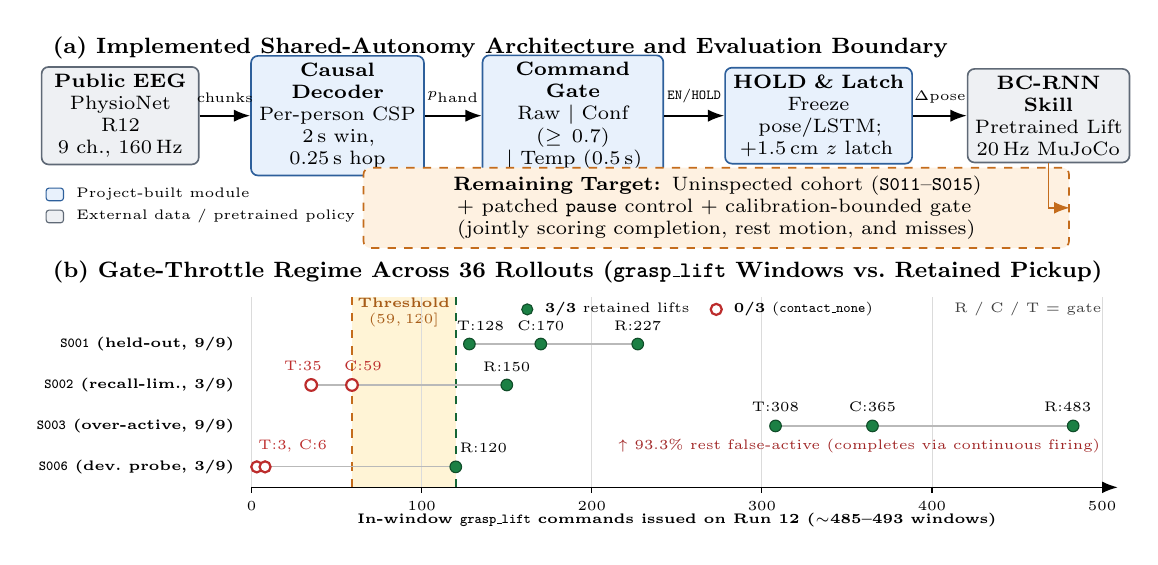
\begin{tikzpicture}[>=Latex, font=\scriptsize]

% ==================== PANEL (A): ARCHITECTURE ====================
\node[anchor=west, font=\footnotesize\bfseries] at (0.0, 2.48) {(a) Implemented Shared-Autonomy Architecture and Evaluation Boundary};

\tikzset{
  pbox/.style={draw=stageborder, line width=0.6pt, rounded corners=2.5pt, fill=stageblue, align=center, minimum height=0.98cm, inner sep=2.5pt},
  ebox/.style={draw=extborder, line width=0.6pt, rounded corners=2.5pt, fill=extgray, align=center, minimum height=0.98cm, inner sep=2.5pt},
  fbox/.style={draw=planborder, line width=0.6pt, dashed, rounded corners=2.5pt, fill=planorange, align=center, minimum height=0.58cm, inner sep=3pt}
}

% Total horizontal span strictly [0.00, 13.78] cm (< 13.97 cm textwidth)
% 5 boxes with generous ~0.72 cm arrow gaps:
% Box 1: [0.00, 1.96] center 0.98
% Gap 1: 0.70 cm
% Box 2: [2.66, 4.82] center 3.74
% Gap 2: 0.78 cm
% Box 3: [5.60, 7.86] center 6.73
% Gap 3: 0.82 cm
% Box 4: [8.68, 11.02] center 9.85
% Gap 4: 0.74 cm
% Box 5: [11.76, 13.78] center 12.77
\node[ebox, text width=1.82cm] (eeg)   at (0.98, 1.62) {\textbf{Public EEG}\\PhysioNet R12\\9 ch., 160\,Hz};
\node[pbox, text width=2.02cm] (dec)   at (3.74, 1.62) {\textbf{Causal Decoder}\\Per-person CSP\\2\,s win, 0.25\,s hop};
\node[pbox, text width=2.12cm] (gate)  at (6.73, 1.62) {\textbf{Command Gate}\\Raw $\vert$ Conf ($\ge\!0.7$)\\$\vert$ Temp (0.5\,s)};
\node[pbox, text width=2.20cm] (latch) at (9.85, 1.62) {\textbf{HOLD \& Latch}\\Freeze pose/LSTM;\\$+1.5$\,cm $z$ latch};
\node[ebox, text width=1.88cm] (robot) at (12.77, 1.62) {\textbf{BC-RNN Skill}\\Pretrained Lift\\20\,Hz MuJoCo};

\draw[->, line width=0.65pt] (eeg) -- node[above, font=\tiny, yshift=1pt]{chunks} (dec);
\draw[->, line width=0.65pt] (dec) -- node[above, font=\tiny, yshift=1pt]{$p_{\text{hand}}$} (gate);
\draw[->, line width=0.65pt] (gate) -- node[above, font=\tiny, yshift=1pt]{\texttt{EN}/\texttt{HOLD}} (latch);
\draw[->, line width=0.65pt] (latch) -- node[above, font=\tiny, yshift=1pt]{$\Delta$pose} (robot);

% Future evaluation bar
\node[fbox, text width=8.75cm] (next) at (8.55, 0.45) {\textbf{Remaining Target:} Uninspected cohort (\texttt{S011}--\texttt{S015}) + patched \texttt{pause} control + calibration-bounded gate (jointly scoring completion, rest motion, and misses)};
\draw[->, line width=0.6pt, draw=planborder] (robot.south) |- (next.east);

% Legend for Panel (a)
\filldraw[fill=stageblue, draw=stageborder, rounded corners=1pt] (0.04, 0.54) rectangle (0.26, 0.70);
\node[anchor=west, font=\tiny] at (0.30, 0.62) {Project-built module};
\filldraw[fill=extgray, draw=extborder, rounded corners=1pt] (0.04, 0.26) rectangle (0.26, 0.42);
\node[anchor=west, font=\tiny] at (0.30, 0.34) {External data / pretrained policy};

% ==================== PANEL (B): EMPIRICAL REGIME PLOT ====================
\node[anchor=west, font=\footnotesize\bfseries] at (0.0, -0.36) {(b) Gate-Throttle Regime Across 36 Rollouts (\texttt{grasp\_lift} Windows vs.\ Retained Pickup)};

% Coordinate mapping: x in [2.65, 13.45] maps commands [0, 500] (span = 10.80 cm)
% x(c) = 2.65 + 10.80 * (c / 500.0)
% c=59  -> 3.924
% c=120 -> 5.242

% Shaded empirical threshold band: (59, 120]
\fill[threshband] (3.924, -3.10) rectangle (5.242, -0.68);
\draw[dashed, draw=planborder, line width=0.55pt] (3.924, -3.10) -- (3.924, -0.68);
\draw[dashed, draw=passgreen!80!black, line width=0.55pt] (5.242, -3.10) -- (5.242, -0.68);
\node[font=\tiny\bfseries, align=center, text=planborder!85!black] at (4.583, -0.88) {Threshold\\$(59,120]$};

% Axes and gridlines
\foreach \c/\xpos in {0/2.65, 100/4.81, 200/6.97, 300/9.13, 400/11.29, 500/13.45} {
  \draw[gray!28, line width=0.35pt] (\xpos, -3.10) -- (\xpos, -0.68);
}

\draw[->, line width=0.6pt] (2.65, -3.10) -- (13.65, -3.10);
\foreach \c/\xpos in {0/2.65, 100/4.81, 200/6.97, 300/9.13, 400/11.29, 500/13.45} {
  \draw (\xpos, -3.10) -- (\xpos, -3.17);
  \node[below, font=\tiny] at (\xpos, -3.16) {\c};
}
\node[font=\tiny\bfseries] at (8.05, -3.52) {In-window \texttt{grasp\_lift} commands issued on Run 12 ($\sim$485--493 windows)};

% Marker legend cleanly spaced at top right of Panel (b)
\filldraw[fill=passgreen, draw=passgreen!60!black] (6.15, -0.84) circle (2.0pt);
\node[anchor=west, font=\tiny] at (6.25, -0.84) {\textbf{3/3} retained lifts};
\filldraw[fill=white, draw=failred, line width=0.8pt] (8.55, -0.84) circle (2.0pt);
\node[anchor=west, font=\tiny] at (8.65, -0.84) {\textbf{0/3} (\texttt{contact\_none})};
\node[anchor=west, font=\tiny, text=black!75] at (11.45, -0.84) {R / C / T = gate};

% Row 1: S001 (y = -1.28): Temp=128 (5.415), Conf=170 (6.322), Raw=227 (7.553) -> ALL 3/3
\node[anchor=east, font=\tiny\bfseries] at (2.55, -1.28) {\texttt{S001} (held-out, 9/9)};
\draw[gray!55, line width=0.45pt] (5.415, -1.28) -- (7.553, -1.28);
\filldraw[fill=passgreen, draw=passgreen!60!black] (5.415, -1.28) circle (2.1pt) node[above, font=\tiny, xshift=4pt, yshift=1.5pt]{T:128};
\filldraw[fill=passgreen, draw=passgreen!60!black] (6.322, -1.28) circle (2.1pt) node[above, font=\tiny, yshift=1.5pt]{C:170};
\filldraw[fill=passgreen, draw=passgreen!60!black] (7.553, -1.28) circle (2.1pt) node[above, font=\tiny, yshift=1.5pt]{R:227};

% Row 2: S002 (y = -1.80): Temp=35 (3.406, 0/3), Conf=59 (3.924, 0/3), Raw=150 (5.890, 3/3)
\node[anchor=east, font=\tiny\bfseries] at (2.55, -1.80) {\texttt{S002} (recall-lim., 3/9)};
\draw[gray!55, line width=0.45pt] (3.406, -1.80) -- (5.890, -1.80);
\filldraw[fill=white, draw=failred, line width=0.8pt] (3.406, -1.80) circle (2.1pt) node[above, font=\tiny, text=failred, xshift=-3pt, yshift=1.5pt]{T:35};
\filldraw[fill=white, draw=failred, line width=0.8pt] (3.924, -1.80) circle (2.1pt) node[above, font=\tiny, text=failred, xshift=4pt, yshift=1.5pt]{C:59};
\filldraw[fill=passgreen, draw=passgreen!60!black] (5.890, -1.80) circle (2.1pt) node[above, font=\tiny, yshift=1.5pt]{R:150};

% Row 3: S003 (y = -2.32): Temp=308 (9.303), Conf=365 (10.534), Raw=483 (13.083) -> ALL 3/3
\node[anchor=east, font=\tiny\bfseries] at (2.55, -2.32) {\texttt{S003} (over-active, 9/9)};
\draw[gray!55, line width=0.45pt] (9.303, -2.32) -- (13.083, -2.32);
\filldraw[fill=passgreen, draw=passgreen!60!black] (9.303, -2.32) circle (2.1pt) node[above, font=\tiny, yshift=1.5pt]{T:308};
\filldraw[fill=passgreen, draw=passgreen!60!black] (10.534, -2.32) circle (2.1pt) node[above, font=\tiny, yshift=1.5pt]{C:365};
\filldraw[fill=passgreen, draw=passgreen!60!black] (13.083, -2.32) circle (2.1pt) node[above, font=\tiny, xshift=-2pt, yshift=1.5pt]{R:483};
\node[anchor=east, font=\tiny, text=failred!85!black] at (13.55, -2.58) {$\uparrow$ 93.3\% rest false-active (completes via continuous firing)};

% Row 4: S006 (y = -2.84): Temp=3 (2.715, 0/3), Conf=6 (2.780, 0/3), Raw=120 (5.242, 3/3)
\node[anchor=east, font=\tiny\bfseries] at (2.55, -2.84) {\texttt{S006} (dev.\ probe, 3/9)};
\draw[gray!55, line width=0.45pt] (2.715, -2.84) -- (5.242, -2.84);
\filldraw[fill=white, draw=failred, line width=0.8pt] (2.715, -2.84) circle (2.0pt);
\filldraw[fill=white, draw=failred, line width=0.8pt] (2.820, -2.84) circle (2.0pt) node[above, font=\tiny, text=failred, xshift=10pt, yshift=1.5pt]{T:3, C:6};
\filldraw[fill=passgreen, draw=passgreen!60!black] (5.242, -2.84) circle (2.1pt) node[above, font=\tiny, xshift=10pt, yshift=1.5pt]{R:120};

\end{tikzpicture}%
}
\caption{\textbf{System overview and midterm empirical regime split.} \textbf{(a)} Project-built modules (blue) connect public motor-imagery EEG to an externally pretrained \texttt{robomimic} \texttt{BC-RNN} policy (gray) via causal decoding, command gating, and a \texttt{HOLD}-preserving completion latch; orange indicates the remaining prospective benchmark. \textbf{(b)} Across 36 learned-policy rollouts (3 scene seeds per gate), cube acquisition and terminal retention separate cleanly across an empirical command-count threshold of $(59, 120]$ \texttt{grasp\_lift} windows, exposing a tradeoff between strict-gate starvation (\texttt{S002}, \texttt{S006}) and unbounded rest false activation (\texttt{S003}).}
\label{fig:pipeline}
\end{figure}

%===============================================================================
\section{Reflection: Where are we?}

\textbf{EEG decoding and scripted baseline.} We built a leakage-safe MNE preprocessing and causal replay pipeline calibrating per-person models on runs 4 and 8 with run 12 held out (9 sensorimotor channels, 8--30\,Hz, 2.0\,s windows). On participants \texttt{S001}--\texttt{S005} (150 test windows), individual CSP/LDA reached 70.67\% balanced accuracy (29.33\% rest false activation), whereas subject-pooled CSP/LDA dropped to 49.33\%; Riemannian tangent-space classification reached 72.67\% individual and 70.00\% pooled accuracy. On a separate five-person cohort (\texttt{S006}--\texttt{S010}), individual CSP/LDA scored 59.33\% balanced accuracy (29.33\% rest false activation). Driving a frozen \emph{scripted} Franka lift over 120-second replays after fixing an initial \texttt{HOLD}-drift bug, raw, confidence ($\ge\!0.7$), and temporal ($0.5$\,s persistence) gates achieved physical lifts in 5/5, 3/5, and 2/5 subjects, respectively. Filtering reduced mean rest command activation from 38.7\% to 25.7\% and 19.6\% (and physical rest motion from 13.5\% to 9.1\%), but increased missed imagery bouts from 12 to 30 and 38.

\textbf{Robot learning progression and pivot.} Custom policy learning in Isaac Lab proved substantially harder than anticipated. While our PPO agent lifted from privileged in-hand resets, ready-pose table transfer yielded 0/5 pickups. Subsequent curriculum variants reached 2/5 lifts in a fixed near-table progress screen (with one drop and asymmetric right-finger contact peaks of 92--169\,N that knocked the cube sideways) and peaked at 3/5 sustained bilateral acquisitions in a unilateral near-table screen, still short of reliable ready-pose pickup or validated \texttt{HOLD} invariance. Rather than stalling the interface study on fragile reward shaping, we integrated an attributed, externally pretrained \texttt{robomimic} \texttt{BC-RNN} Panda Lift policy~\citep{mandlekar2021} in native MuJoCo. Naive intermittent gating initially retained the cube in 0/5 terminal states; engineering a stateful adapter that freezes both the end-effector target and recurrent hidden state during \texttt{HOLD}, paired with a one-time $+1.5$\,cm world-$z$ goal offset at bilateral grasp acquisition, achieved 21/21 retained lifts across positive development controls and 0/3 on \texttt{always-hold} negatives.

\textbf{Connected EEG-to-learned-policy results.} We then executed 36 offline decision-stream rollouts (400 steps / 20\,s at 20\,Hz; seeds 0--2 per gate) across exploratory subject \texttt{S006} and all three held-out subjects \texttt{S001}--\texttt{S003}, bracketed on \texttt{S001} by matched \texttt{always-enable} (3/3 retained, steps 47--58) and \texttt{always-hold} (0/3) controls:
\begin{itemize}
  \item \textbf{Balanced held-out (\texttt{S001}, 76.7\% BA, 20.0\% rest false-active):} Completed and retained \textbf{9/9} lifts across raw (227 commands), confidence (170), and temporal (128) gates with zero drops.
  \item \textbf{Recall-limited (\texttt{S002}, 73.3\% BA, 53.3\% hand recall; and exploratory \texttt{S006}):} Completed \textbf{3/9} each---retaining 3/3 under raw commands (\texttt{S002}: 150; \texttt{S006}: 120) but 0/3 under confidence (\texttt{S002}: 59; \texttt{S006}: 6) and temporal (\texttt{S002}: 35; \texttt{S006}: 3) gates, which starved the policy of reach time.
  \item \textbf{Precision-limited (\texttt{S003}, 53.3\% BA, 93.3\% rest false-active):} Completed \textbf{9/9} lifts across all three gates (483/365/308 commands), succeeding physically because near-continuous false firing acted like an always-on trigger.
\end{itemize}

\textbf{Was the gap real, did we verify our insight, and what was harder than expected?} The gap between offline decoding and closed-loop utility proved sharper than hypothesized, though as an empirical systems problem rather than an unstudied paradigm~\citep{akinola2017,carrara2023}. Uncalibrated LDA posteriors caused fixed-threshold ($\ge\!0.7$) duty cycles to swing nearly $50\times$ across individuals (0.012 on \texttt{S006} vs.\ 0.565 on \texttt{S008}), making offline accuracy a poor predictor of completion: \texttt{S002} (73.3\% BA) failed filtered gates, whereas \texttt{S003} (53.3\% BA) completed every rollout via unintended rest activation. Our shared-autonomy insight is verified in bounded form---binary EEG replay can drive a learned manipulation skill when mediated by a recurrent-state-preserving \texttt{HOLD} and grasp latch---while falsifying our naive assumption that fixed temporal filtering uniformly helps. Three engineering subtleties were harder than expected: sustaining bilateral contact through terminal states rather than brief reward spikes, preventing \texttt{HOLD} target drift, and auditing control baselines---where a code review caught and patched an inverted \texttt{pause}-matched control branch (\texttt{hold} vs.\ \texttt{policy} inside the timed window) before any invalid causal localization was claimed.

%===============================================================================
\section{Updated work plan}

To guarantee a rigorous, self-contained project by semester end, we pivot from training manipulation policies from scratch to a controlled shared-autonomy systems benchmark around the attributed \texttt{BC-RNN} controller. Because fixed confidence thresholds either starve conservative decoders or reward over-active ones, we also add a lightweight, calibration-only quantile/conformal gate threshold (fit strictly on runs 4 and 8 to target bounded rest false activation) alongside our frozen gates.

\begin{table}[h]
\centering
\caption{Revisions from the initial twelve-week proposal to the final semester plan.}
\label{tab:plan}
\footnotesize
\begin{tabular}{@{}>{\raggedright\arraybackslash}p{0.25\linewidth}>{\raggedright\arraybackslash}p{0.15\linewidth}>{\raggedright\arraybackslash}p{0.54\linewidth}@{}}
\toprule
\textbf{Original component} & \textbf{Status} & \textbf{Revision and technical rationale} \\
\midrule
EEG baselines \& replay & Complete & Per-person/pooled CSP and Riemannian pipelines plus causal replay verified; retain binary \texttt{T0} vs.\ \texttt{T1}/\texttt{T2} labels. \\
Isaac Lab PPO table pickup & Stopped & Best near-table policy reached 3/5 lifts with asymmetric impact forces; retire custom RL and use attributed \texttt{robomimic} \texttt{BC-RNN}. \\
\texttt{HOLD} \& retention adapter & Complete & Added state-freezing \texttt{HOLD} executor and $+1.5$\,cm latch (21/21 dev.\ controls); patched inverted \texttt{pause}-control bug. \\
Learned-policy EEG replay & Held-out (\texttt{S001}--\texttt{S003}) & 24/36 retained lifts across \texttt{S001}--\texttt{S003} and \texttt{S006} revealed the $(59,120]$ trigger threshold; expand to uninspected cohort. \\
Fine gestures \& hardware & Deferred & Dataset lacks grasp/wrist labels; replace extra deep architectures with calibration-bounded gating and matched controls. \\
\bottomrule
\end{tabular}
\end{table}

\textbf{Remaining schedule (Weeks of Nov.\ 9 -- Dec.\ 7).}
\textbf{(1) Nov.\ 9:} Execute the corrected \texttt{pause}-matched timing controls on \texttt{S001}--\texttt{S003} to isolate duty-cycle sufficiency from fragmented EEG timing, and freeze all code hashes, unseen scene seeds, and per-person calibration rules (runs 4/8 only) before opening new subjects.
\textbf{(2) Nov.\ 16--23:} Run a single prospective evaluation on five uninspected PhysioNet participants (\texttt{S011}--\texttt{S015}, run 12) comparing raw, fixed-confidence, temporal, and calibration-bounded gates against \texttt{always-hold}, \texttt{always-enable}, and duration-matched \texttt{pause} controls without post-hoc window selection.
\textbf{(3) Nov.\ 30:} Join EEG cue annotations to MuJoCo telemetry to jointly score retained completion, robot motion during annotated rest, missed imagery bouts, and detection latency, testing whether calibration-bounded gating curbs \texttt{S003}-style rest motion without inducing \texttt{S002}-style starvation.
\textbf{(4) Dec.\ 7:} Deliver the final report, synchronized trace-and-rollout video, and one-command reproduction scripts. If uninspected subjects fail to acquire, we will report the exact failure mechanism without relaxing thresholds; offline replay will not be represented as live closed-loop BCI or clinical validation.

%===============================================================================
\section{AI statement}

AI coding and writing assistants (OpenAI Codex, Claude, and Google Antigravity) were used to help organize literature metadata, scaffold simulation/evaluation scripts, audit control harnesses, summarize logged telemetry, and refine the prose and TikZ figure in this report. All numerical claims, SHA-256 artifact records, and experimental interpretations were verified against saved repository outputs, externally pretrained models are explicitly attributed, and full responsibility for the technical conclusions and limitations rests with the author.

\bibliography{references}

\end{document}
